\section{Generative Speech Reward Model} \label{sec:gsrm}

\begin{figure*}[!t]
    \centering
    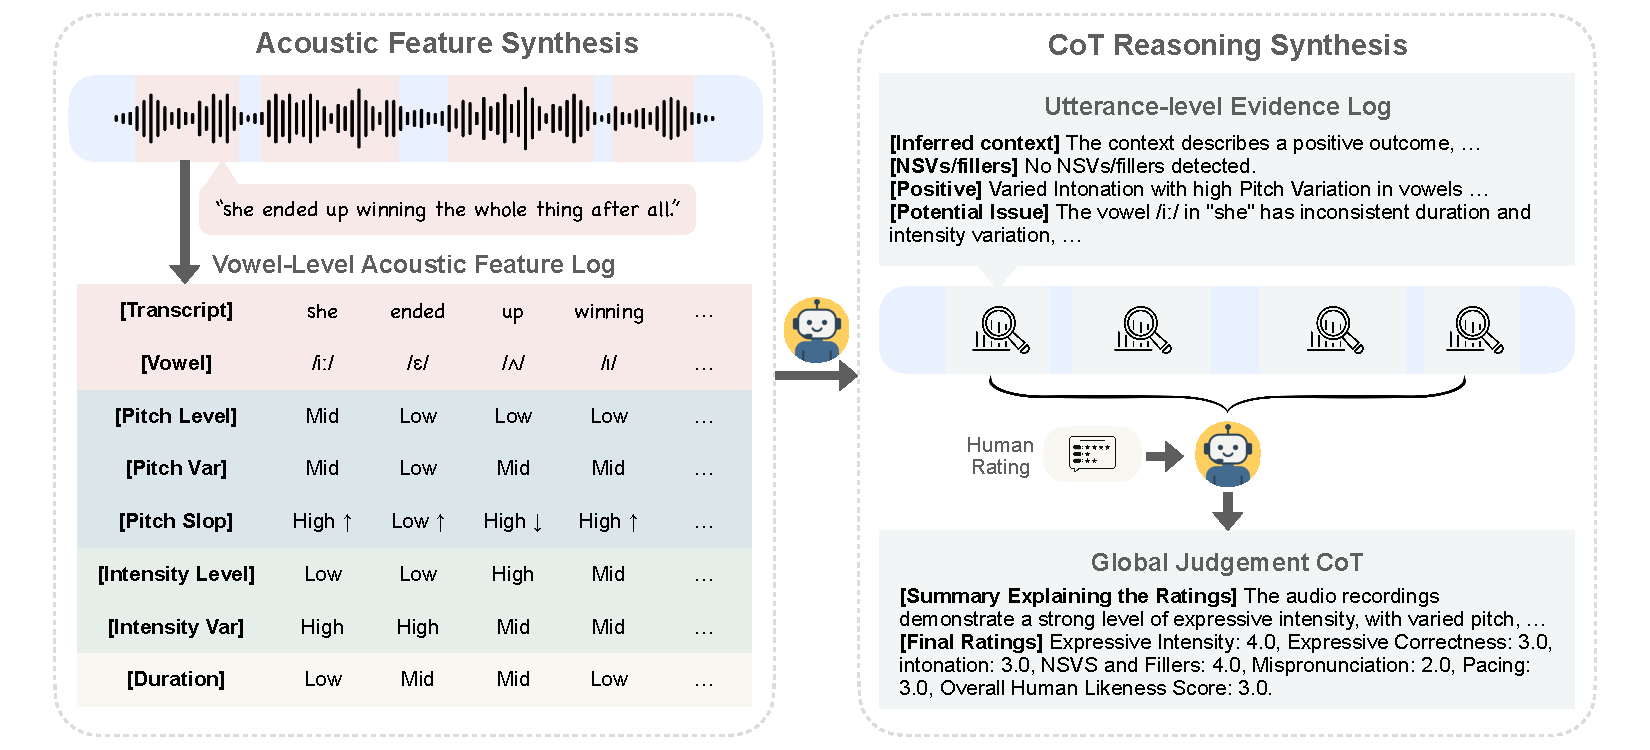
\includegraphics[width=1.0\textwidth]{Figures/teaser.pdf}
\caption{\textbf{CoT Synthesis Framework of GSRM.} For each utterance segment, the synthesis pipeline first extracts structured, vowel-level acoustic features from the segment and then synthesizes detailed reasoning to connect paralinguistic cues with perceptual judgments. This process is applied across all utterance segments to construct a complete evidence log for the audio, which is subsequently combined with a global judgment CoT to form the final training trajectory for training GSRM.}
\label{fig:teaser}
\vspace{-0.5em}
\end{figure*}

Our ultimate goal is to build a \emph{generative reward model} tailored for speech, which first extracts inherent paralinguistic evidence from speech and then reasons over this evidence to judge audio quality. While our focus is speech naturalness evaluation, GSRM is designed as a universal framework that can assess any attribute of speech through reasoning. At a high level, GSRM emulates the human evaluation process: human raters implicitly attend to prosodic cues such as pitch movement, loudness variation, and timing, synthesize these observations into quantitative judgments of overall naturalness. To train GSRM to achieve this, we need two stages: (i) extracting structured acoustic features from the raw audio for downstream judgment, and (ii) synthesizing explicit chain-of-thought (CoT) reasoning trajectories that connect these features to quantitative ratings.

\begin{table*}[h]
\centering
\renewcommand{\arraystretch}{1.2}
\setlength{\tabcolsep}{10pt}
\footnotesize
\caption{\textbf{Acoustic Features.}
Vowel-level prosodic features extracted from time-aligned vowel segments, serve as sufficient statistics for speech naturalness judgment.}
\vspace{-0.6em}

\begin{tabular}{p{2.2cm} p{12.6cm}}
\toprule
\textbf{Acoustic Feature} & \textbf{Definition and Interpretation} \\
\midrule
\textbf{Pitch Level} &
Average fundamental frequency ($F_0$) of a vowel segment, reflecting overall pitch height. \\

\textbf{Pitch Var.} &
Within-segment variability of frequency, reflecting the degree of expressiveness. \\

\textbf{Pitch Slope} &
Trend of frequency change across the vowel segment (rising or falling), reflecting local intonation contours. \\

\textbf{Intensity Level} &
Average loudness (e.g., RMS energy) of the vowel segment, reflecting perceived vocal strength or emphasis. \\

\textbf{Intensity Var.} &
Temporal fluctuation of intensity within the vowel segment, indicating stability or variability in loudness. \\

\textbf{Duration} &
Temporal length of the vowel segment, reflecting speech rate, emphasis, and pacing characteristics. \\

\bottomrule
\end{tabular}
\label{table:acoustic-features}
\vspace{-0.5em}
\end{table*}


\begin{table*}[!t]
\centering
\renewcommand{\arraystretch}{1.25}
\setlength{\tabcolsep}{10pt}
\captionsetup{font=small}
\footnotesize
\caption{\textbf{Evidence Log Dimensions.}
Each utterance is analyzed along four dimensions to synthesize interpretable reasoning grounded in acoustic features and transcript context.}
\vspace{-0.6em}

\begin{tabular}{p{2.4cm} p{12.6cm}}
\toprule
\textbf{Dimension} & \textbf{Description} \\
\midrule
\textbf{Inferred Context} &
A concise description of the communicative intent of the utterance (e.g., question, acknowledgment, neutral statement), inferred from the transcript. \\

\textbf{NSVs / Fillers} &
Identification of any non-speech vocalizations or filler words (e.g., ``yeah'', ``uh'',  ``uh''), supported by transcripts and acoustic feature such as abrupt pitch or intensity variation. \\

\textbf{Positive Attributes} &
Identification of perceptual strengths, such as appropriate emphasis, smooth intonation, or natural fillers, grounded in specific vowels and their acoustic features. \\

\textbf{Potential Issue} &
Identification of perceptual weaknesses, including intonation instability, pacing inconsistency, expressive incorrectness, or unnatural pauses, grounded in specific vowels and their acoustic features.  \\

\bottomrule
\end{tabular}
\label{table:cot-dimensions}
\vspace{-1em}
\end{table*}

\textbf{Acoustic Feature Extraction.} Judging speech naturalness directly from raw audio is challenging due to the high dimensionality and redundancy of waveform signals. From an information-theoretic perspective, raw audio contains more information than is required to infer perceptual naturalness ratings. We therefore assume the existence of a set of \emph{sufficient statistics}~\cite{cover1999elements} that preserves all information relevant to naturalness judgment while discarding redundancy. In the context of speech evaluation, such sufficient statistics naturally correspond to a set of interpretable acoustic features. Specifically, we adopt a vowel-level acoustic feature extraction pipeline. Given an audio recording and its transcript, we perform phoneme-level forced alignment to obtain precise temporal boundaries for each phoneme, and retain only vowel segments. This is motivated by the observation that vowels, as voiced and acoustically stable units, carry the majority of prosodic information relevant to expressiveness, intonation, and pacing.

As shown in Figure~\ref{fig:teaser}, for each vowel segment, we extract a compact set of low-level prosodic features as summarized in Table~\ref{table:acoustic-features}. To improve robustness and interpretability, continuous feature values are discretized into ordinal categories (e.g., very low, low, mid, high, very high). After feature extraction, we obtain a raw \emph{acoustic feature log} structured at the utterance level. For each utterance, the log records detailed vowel-level acoustic analyses across the entire utterance, which serve as the main evidence for subsequent reasoning and naturalness judgment.

\textbf{Reasoning Synthesis.} While acoustic features capture essential paralinguistic evidence, they do not, by themselves, specify how such evidence should be interpreted to form perceptual judgments of speech naturalness. Bridging this gap requires the synthesis of CoT reasoning that maps acoustic cues to ratings of each evaluation metrics and overall human-likeness. As shown in Figure~\ref{fig:teaser}, for each utterance in the raw \emph{acoustic feature log}, we provide a frontier text model (GPT-4o) with the utterance transcript and its associated vowel-level acoustic features. The model is prompted to generate a structured analysis along four dimensions: inferred conversational context, identification of non-speech vocalizations or fillers, positive perceptual attributes, and potential issues (see Table~\ref{table:cot-dimensions}). This process produces an \emph{utterance-level evidence log} that articulates how local prosodic patterns contribute to qualitative perceptual impressions. In the second stage, we synthesize a \emph{global judgment CoT} that maps the entire utterance-level evidence log to final human ratings. The model is provided with both the evidence log and the oracle human ratings, and is instructed to generate a coherent assessment explaining how the observed evidence supports the assigned scores. The final CoT trajectory used for training is obtained by concatenating the \emph{utterance-level evidence log} with the synthesized \emph{global judgment CoT}. 

\textbf{Training and Deployment.} We synthesize CoT trajectories for all samples in the ConvTTS training set to construct the training data for GSRM. We then fine-tune Qwen2.5-Omni-7B to take raw audio as input and generate the corresponding synthesized CoT trajectories via supervised fine-tuning (SFT). Through this procedure, the model is encouraged to learn not only \emph{what} ratings to assign, but also \emph{why} those ratings are justified given the underlying acoustic evidence. In addition, we explore whether reinforcement learning with verifiable rewards (RLVR) can further improve naturalness prediction performance. The discussion is provided in Appendix~\ref{sec:gsrm_rl}. Once trained, GSRM is deployed in the same manner as a speech-in, text-out LLMs. Given a raw audio recording, GSRM produces a textual CoT reasoning, followed by numerical ratings for individual sub-metrics as well as an overall human-likeness score. To improve robustness, we further employ test-time scaling by sampling multiple random predictions for the same audio input and averaging the resulting scores. Empirically, we observe that using more test-time samples consistently improves model–human consistency (see Section~\ref{sec:main_results}).
